% 图 17.1 —— **手写重建版**（推翻原「描摹稿」；用户 2026-10-08 裁定「描摹稿要全部推翻重来」）
%
% 内容 = 外矩形 + 左上白框（**内部是花的**）+ 右下白框（**内部是白的**）+ 标签 Y A C X。
%
% ★★ 叠放次序（用户 2026-10-08 口述，已与原书逐块核对坐实）：
%     ① **先画左上的框**（只画轮廓，不填白）
%     ② **再满铺阴影** —— 阴影因此盖过左上框的内部 ⇒ **左上框里是花的**
%     ③ **最后画右下的框**（白底 + 轮廓）—— 白底盖住阴影 ⇒ **右下框里是白的**
%   ⇒ 两框的**交叠小方块**落在右下框之内 ⇒ **也是白的**（与书一致，见 `_zR2` 核对）
%   ★ 小方块是"交叠围出来的"，**不单独画**。
%
% ★ 标签 **Y 与 C 要加白底**：Y 在左上框**左外侧**、C 在右下框**右外侧**，
%   两者都落在**阴影区**里，不加白底会被斜线穿字。`A` 在交叠块（白区）内，不需要。
%
% 几何**实测**自 `images/17.1.png`（与本画布 1:1，非描摹）：
%   外矩形  x[16.0, 458.5]  y[20.5, 357.5]
%   左上框  x[90.5, 286.5]  y[67.0, 220.0]
%   右下框  x[232.5, 355.5] y[144.0, 327.5]
%
% 线宽：轮廓与阴影线**各一档**（原描摹稿是 9 档）。
\documentclass[12pt]{standalone}
\usepackage{fontspec}
\setsansfont{Arial}
\newfontfamily\mfallback{DejaVu Sans}
\usepackage{tikz}
\usetikzlibrary{patterns}

% ── 阴影线：45°，垂直线间距 13pt，线宽 3.3pt（与原书实测 12.7 / 3.2 一致；同图 1.1）──
\pgfdeclarepatternformonly{hatch45}
  {\pgfqpoint{-18.385pt}{-18.385pt}}
  {\pgfqpoint{18.385pt}{18.385pt}}
  {\pgfqpoint{18.385pt}{18.385pt}}
  {\pgfsetlinewidth{3.3pt}\pgfsetstrokecolor{black}%
   \pgfpathmoveto{\pgfqpoint{0pt}{0pt}}%
   \pgfpathlineto{\pgfqpoint{18.385pt}{18.385pt}}%
   \pgfusepath{stroke}}

\def\wEdge{5.0}
\def\wHatch{3.3}

\begin{document}
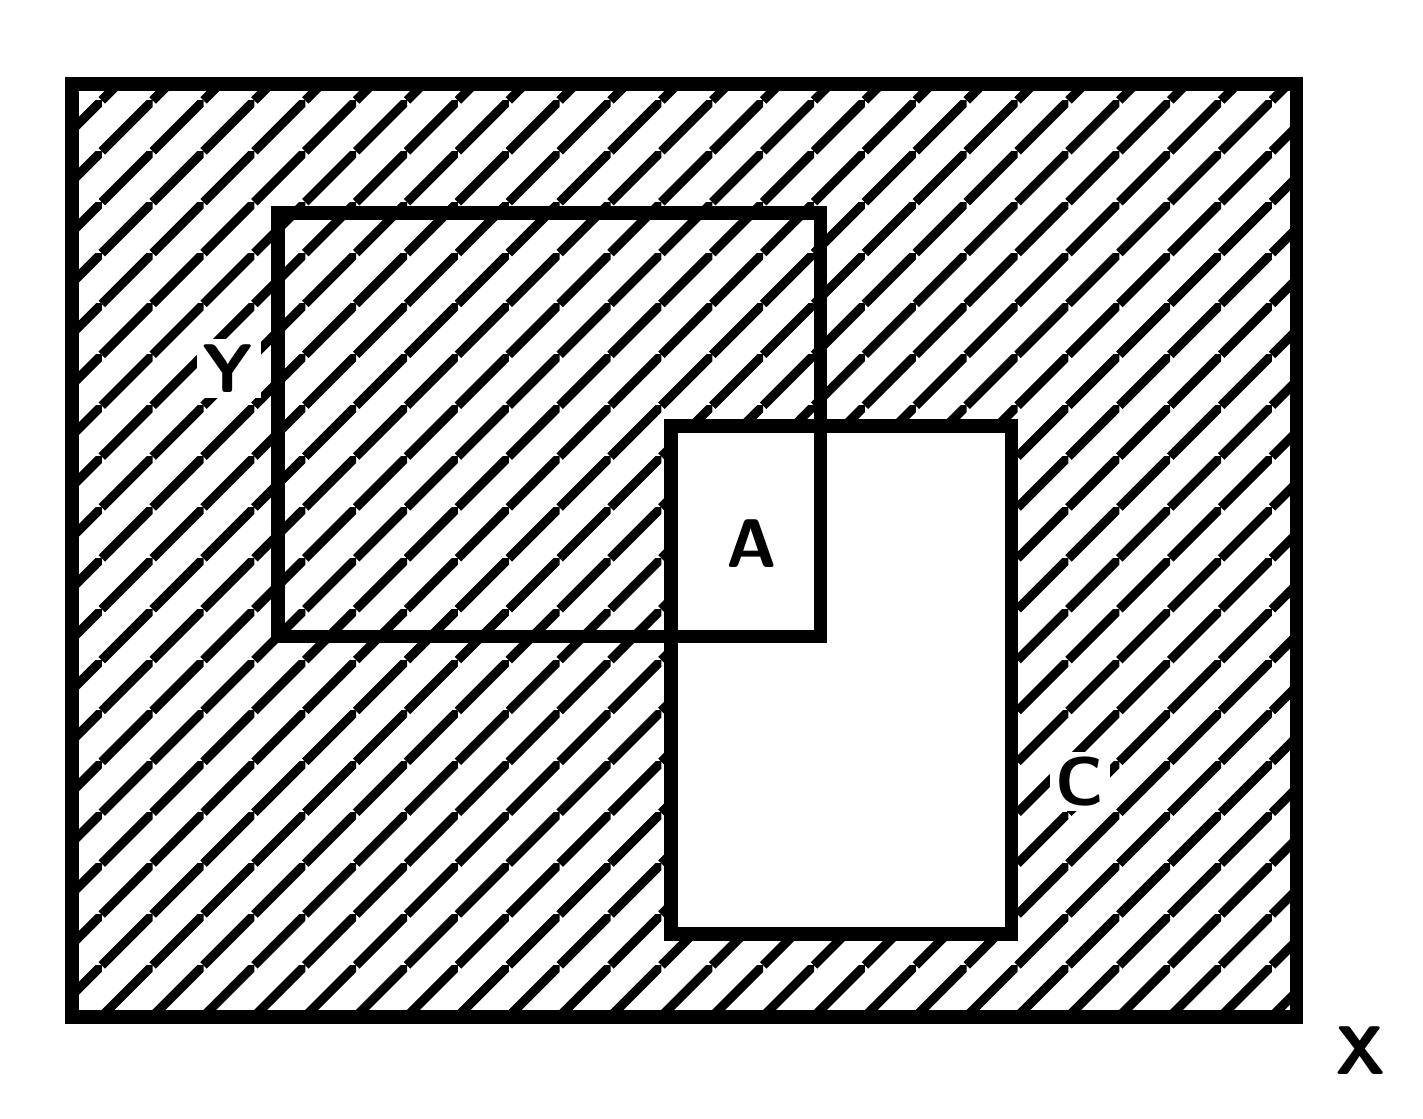
\begin{tikzpicture}[x=1pt, y=-1pt, line width=\wEdge, line cap=butt, line join=miter]

  %% ════ 几何（实测，见文件头）════
  \def\Xa{16.0}  \def\Xb{458.5} \def\Ya{20.5}  \def\Yb{357.5}   % 外矩形
  \def\Pa{90.5}  \def\Pb{286.5} \def\Qa{67.0}  \def\Qb{220.0}   % 左上框
  \def\Ra{232.5} \def\Rb{355.5} \def\Sa{144.0} \def\Sb{327.5}   % 右下框

  %% ① 满铺阴影（左上框**不填白** ⇒ 它的内部保持花的）
  \begin{scope}
    \clip (\Xa,\Ya) rectangle (\Xb,\Yb);
    \fill[pattern=hatch45] (\Xa,\Ya) rectangle (\Xb,\Yb);
  \end{scope}

  %% ② 右下框的白底（盖住阴影 ⇒ 内部是白的；交叠块落在它之内 ⇒ 也是白的）
  \fill[white] (\Ra,\Sa) rectangle (\Rb,\Sb);

  %% ③ **三条轮廓一律画在最上层**
  %%    ⚠ 左上框的轮廓若画在②之前，会被右下框的白底吃掉 ⇒ **交叠小方块的左边/上边会缺**。
  %%      原书里小方块的四条边都在（左上框的右/下边 + 右下框的左/上边）。
  \draw (\Xa,\Ya) rectangle (\Xb,\Yb);   % 外框
  \draw (\Pa,\Qa) rectangle (\Pb,\Qb);   % 左上框（先画的那个，只补轮廓）
  \draw (\Ra,\Sa) rectangle (\Rb,\Sb);   % 右下框

  %% ════ 标签（位置=原书实测字形框中心；字符已核过，一字未改）════
  \node[anchor=center,inner sep=2pt,fill=white,font=\fontsize{29.8}{37.3}\selectfont] at (72.7,123.2) {\textsf{\textbf{\textit{Y}}}};
  \node[anchor=center,inner sep=0pt,font=\fontsize{28.8}{36.0}\selectfont] at (261.6,186.5) {\textsf{\textbf{\textit{A}}}};
  \node[anchor=center,inner sep=2pt,fill=white,font=\fontsize{31.3}{39.2}\selectfont] at (380.3,272.3) {\textsf{\textbf{\textit{C}}}};
  \node[anchor=center,inner sep=0pt,font=\fontsize{38.1}{47.6}\selectfont] at (481.8,369.5) {\textsf{\textbf{\textit{X}}}};

  % 钉死画布
  \pgfresetboundingbox
  \path[use as bounding box] (0,0) rectangle (494,384);
\end{tikzpicture}
\end{document}
